% Describe what we are gonna do, the general ideas and what we are gonna talk about.
% Say what is needed to understand the sections that will follow.

The purpose of the project 
is the evaluation of the performances variation of a wireless network 802.11 b/g at the change of some parameters.
\\\newline
In order to make those tests we used some tools which are Iperf, wireshark, and a complex python script for the automated run test.
\\\newline
The test basicaly consists of many automatic executions of iperf with fixed time and different speed, and finaly we consider the amount of transfering data.
\\\newline
The set of the tests was an indoor environment: one notebook which runs iperf as server, another one which runs iperf as client (through the python script), a cisco access point and another notebook wich runs wireshark to capture the traffic.

\vspace{1cm}

\begin{figure}[h!]
	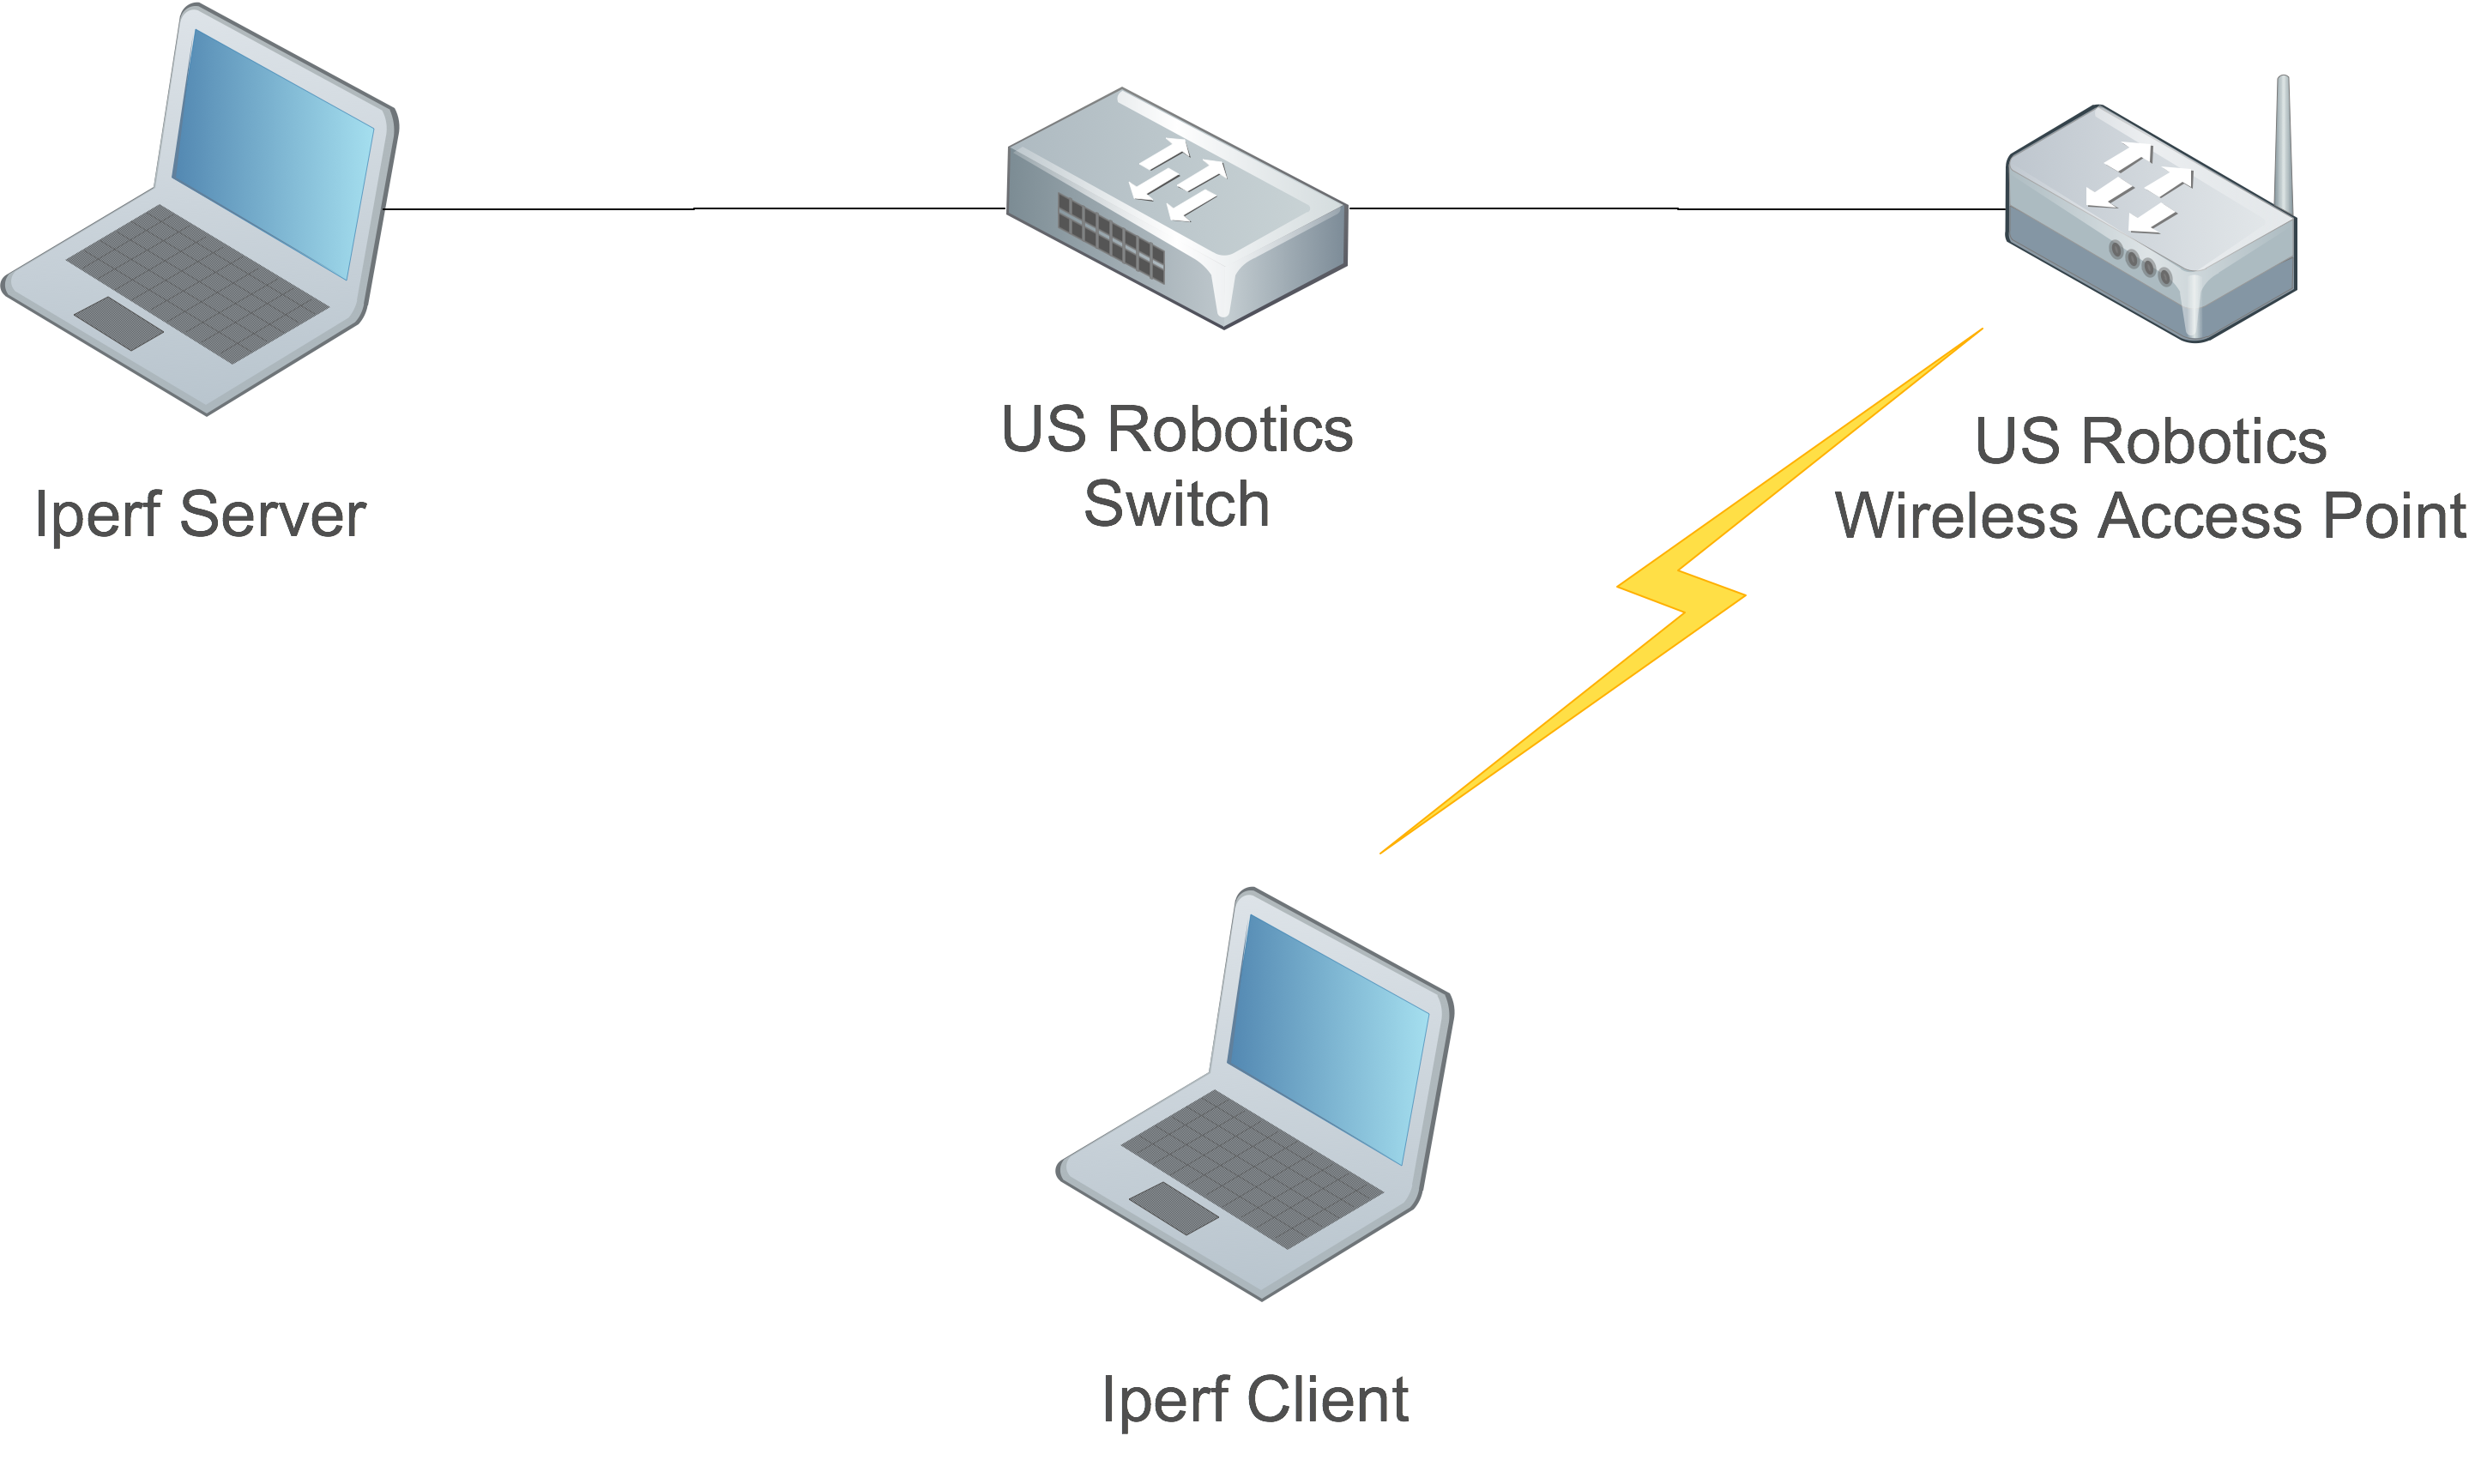
\includegraphics[angle=0, keepaspectratio=true, width=15cm]{../images/network_overview}
	\caption{Network overview}
\end{figure}
